%  Versión 2021
%

% Capítulo 4. Instrumentos de control
% 4.1.      Indicación de la cantidad de combustible, eléctrica y electrónica
% 4.2.      Indicadores de posición a distancia de CC y CA.
% 4.3.      Termómetros, diferentes tipos de lectura directa y a distancia
% 4.4.      Medidores de presión, diferentes tipos de lectura directa y a distancia.

\chapter{Instrumentos de Control}
\label{chap:U04.instrumentos.ctrol}

% \section{Introduccion}
% \label{sec:U04.00.introduccion}


% \section{Indicación de la cantidad de combustible, eléctrica y electrónica}
% \label{sec:U04.01.indicacion.cantidad.combustible}


\section{Indicadores de posición a distancia de CC y CA}
\label{sec:U04.02.indicadores.posicion.a.distancia.cc.ca}

\begin{flushright}
  Por el Prof. Ing. Pedro Giraudo
\end{flushright}



  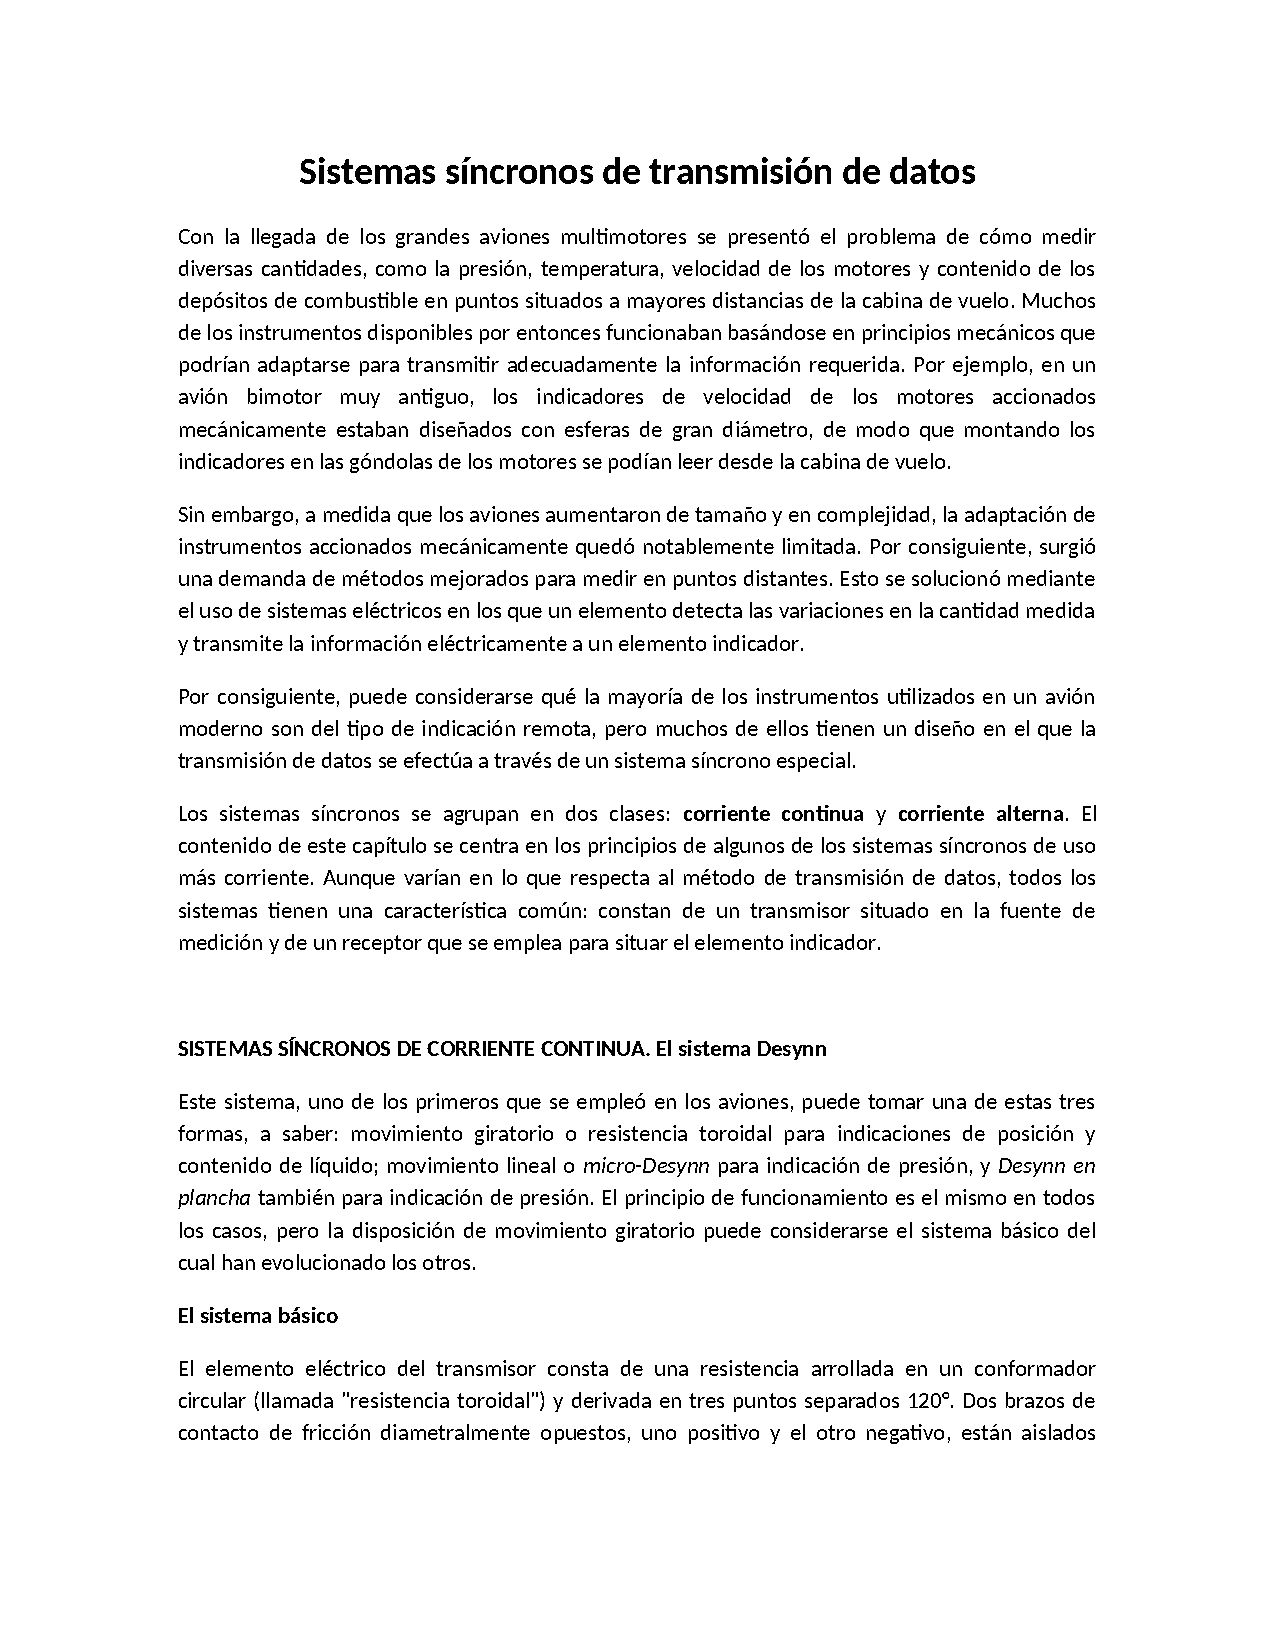
\includepdf[pages=-, fitpaper=false, scale=1.0, %landscape=true,
  offset = 0 -20,
  pagecommand={\thispagestyle{fancy}}]
{04.instrumentos.ctrol/SistemasSincronosDeTransmisionDeDatos.pdf}

% \section{Termómetros, diferentes tipos de lectura directa y a distancia}
% \label{sec:U04.03.termometros}


% \section{Medidores de presión, diferentes tipos de lectura directa y a distancia}
% \label{sec:U04.04.medidores.presion}

